\documentclass[11pt]{article}

\usepackage[margin=1in]{geometry}
\usepackage{amsmath,amssymb}
\usepackage{graphicx}
\usepackage{booktabs}
\usepackage{array}
\usepackage{xcolor}
\usepackage{tikz}
\usetikzlibrary{arrows.meta,positioning,fit,backgrounds}
\usepackage[hidelinks]{hyperref}
\usepackage{caption}
\captionsetup{font=small,labelfont=bf}
\usepackage{titlesec}
\titlespacing*{\section}{0pt}{1.2em}{0.5em}
\titlespacing*{\subsection}{0pt}{0.9em}{0.4em}

\newcommand{\ttt}[1]{\texttt{\small #1}}
\definecolor{ipsi}{RGB}{31,119,180}
\definecolor{contra}{RGB}{214,39,40}
\definecolor{stagebox}{RGB}{235,242,250}
\definecolor{confirm}{RGB}{40,120,60}
\definecolor{caveat}{RGB}{180,120,0}

\title{\vspace{-1.5em}\textbf{Verifying and Resolving the Figure--Ground Circuit's\\
Wing--Steering Output: A Closed-Loop Agentic Connectome Trace\\
of Descending-Neuron Projections to Both Wings in \emph{Drosophila}}}
\author{}
\date{}

\begin{document}
\maketitle
\vspace{-3em}

\begin{abstract}
\noindent
The connectomic study \emph{Finding Vision--Behavior Circuit through Connectomics}
(Ziyin, \ldots, Poggio; herein the \emph{source paper}) traced a figure--ground / course-control
circuit in the adult \emph{Drosophila} brain: a centrifugal horizontal cell (VCH) presynaptically
gates the T4/T5 terminals that drive a retinotopic cholinergic LLPC1 sheet, whose figure signal is
read out by the Nod1 relay and routed to descending neurons (DNs). For the seven figure-driven DNs,
the source paper reported each DN's wing-steering output split by ipsilateral versus contralateral
wing (its Table~S14) and gave DNp26's strongest steering-muscle targets (its Table~S15), as
summary values in a manuscript table. Here we (i) \emph{independently reproduce} those values from
the connectome and (ii) make the underlying \mbox{DN $\rightarrow$ motor neuron $\rightarrow$ wing
muscle} map explicit at per-edge, both-wings resolution. We do this with a closed-loop, steerable,
multi-agent system that proposes a motif, extracts it from the connectome, verifies it against the
source paper's tables, and certifies results only if they pass a strict gate (no refuted claims;
both-wing coverage for every seed DN). The system reproduces every sampled value of S14/S15 exactly,
and emits a machine-readable \mbox{$488$-edge}, \mbox{$139$-motor-neuron}, \mbox{$69$-muscle}
bilateral dataset---the per-edge wiring behind the source paper's summary tables---with $26$ confirmed
and $3$ caveated claims and \emph{zero} refutations. The contribution is threefold: independent
verification of the source paper's wing-steering output, a per-edge bilateral dataset that the
manuscript reported only in aggregate, and the agentic method that produced both under a verification
gate. The resolved map shows how a single retinotopic figure representation issues bilateral
(DNbe001), purely ipsilateral (DNa04), and contralateral single-wing (DNp26, DNg32, DNge094) steering
commands onto identified wing muscles.
\end{abstract}

\section{Background: the figure--ground circuit and its motor output}

The source paper established a two-stage architecture for how a fly converts local object motion into
flight course-control while suppressing self-induced optic flow:

\begin{itemize}\itemsep1pt
\item \textbf{Stage 1 (separation).} The GABAergic centrifugal horizontal cell \textbf{VCH} pools
wide-field T4/T5 motion and feeds inhibition back onto the very T4/T5 terminals that drive the readout
sheet, presynaptically gating common-mode motion before the sheet is reached.
\item \textbf{Stage 2 (readout and steering).} The cholinergic, retinotopic \textbf{LLPC1} sheet reads
out the gated local signal and routes it---dominantly through the \textbf{Nod1} relay---to descending
neurons, of which the strongest direct target is \textbf{DNbe001} and the principal convergent
steering command is \textbf{DNp26}.
\end{itemize}

\noindent
The source paper then asked where this signal reaches motor control. Using the male whole-CNS
connectome (MCNS), it identified seven figure-driven DN types whose dominant motor system is
wing-steering and, in its Table~S14, reported for each the fraction of wing-steering output reaching
the ipsilateral versus the contralateral wing (some drive the ipsilateral wing, some the
contralateral, some both), and in its Table~S15 gave DNp26's strongest steering-muscle targets (the
contralateral \ttt{hg1}, \ttt{i1}, \ttt{hg2}). These were published as \emph{summary values in
manuscript tables}: per-DN fractions and top-target lists, not the underlying per-edge wiring.

\textbf{Scope of this work.} We do not claim to discover bilateral structure the source paper lacked:
S14 already gives the ipsi/contra wing split for these DNs. What we contribute is (1) an
\emph{independent reproduction} of S14/S15 directly from the connectome, as a verification of the
source paper's motor-side claims; (2) the \emph{per-edge, both-wings dataset} that underlies those
summary tables---every DN$\rightarrow$motor-neuron$\rightarrow$muscle edge with its wing side, rather
than the aggregate fraction; and (3) the \emph{closed-loop agentic system} that produced and certified
both, under a gate that refuses to report unverified or incompletely-covered results. (Note: the source
paper's ``one-hemisphere exemplar'' caveat concerns the laterality of the analyzed LLPC1 \emph{sheet},
not the DN$\rightarrow$wing split, which S14 reports for both wings.)

\section{A closed-loop, steerable agentic system for connectome circuit tracing}

Rather than hand-curate the extension, we built an autonomous system that treats ``complete the
muscular projection'' as a verifiable, closed-loop search. The design separates a deterministic
scientific pipeline from a model-driven supervisory layer (Fig.~\ref{fig:system}).

\paragraph{Pipeline (per round).} Five gated stages run as a directed pipeline:
\ttt{seed} $\rightarrow$ \ttt{propose} $\rightarrow$ \ttt{extract} $\rightarrow$ \ttt{verify}
$\rightarrow$ \ttt{report}. \emph{Seed} fixes the scientific target (start from DNbe001 + DNp26,
trace to both wings). \emph{Propose} emits a concrete, runnable motif specification. \emph{Extract}
pulls the DN$\rightarrow$MN$\rightarrow$muscle edges from the connectome. \emph{Verify} re-derives
every claim and renders a verdict. \emph{Report} compiles the certified dataset.

\paragraph{The verification gate.} A round's \ttt{verify} stage \emph{completes} only if two
conditions hold: (i) \textbf{no claim is refuted}, and (ii) \textbf{bilateral coverage is complete}
(every seed DN reaches $\geq 1$ wing-steering motor neuron on \emph{both} wings, and the full
DN$\rightarrow$MN$\rightarrow$muscle chain is closed). A refuted edge or a coverage gap fails the
gate---which is the closed-loop signal to re-propose (drop/replace an edge, widen the seed) and run
another round. This makes the loop self-correcting and steerable: a human (or the supervising agent)
can amend the target mid-flight and the next round re-runs against it.

\paragraph{Supervisory layer.} A language-model agent (GLM~5.2) supervises each tick: it runs the
deterministic heartbeat that advances the pipeline, reads the verdicts, and decides
\emph{monitor} / \emph{re-loop} / \emph{escalate}. A hard guardrail forbids the agent from ever
editing the verifier or ``fixing'' a refuted result---a refutation is a scientific outcome, not a bug.
The deterministic heartbeat guarantees the science progresses even if the supervisory layer is
unavailable; the agent adds reasoning, provenance journaling, and human-facing reporting on top.

\paragraph{Verification philosophy.} Every quantitative claim is checked on two independent tracks
(an all-synapse ``published-total'' track and a synapse-thresholded robustness track) and, where the
source paper reports a value, cross-checked against it as an oracle. Laterality claims are additionally
tested against a soma-side label-permutation null. The agent is only permitted to emit the per-edge
dataset after it has reproduced the source paper's summary values---so the resolved map is anchored to
a verified baseline rather than asserted independently.

\begin{figure}[t]
\centering
\resizebox{\textwidth}{!}{%
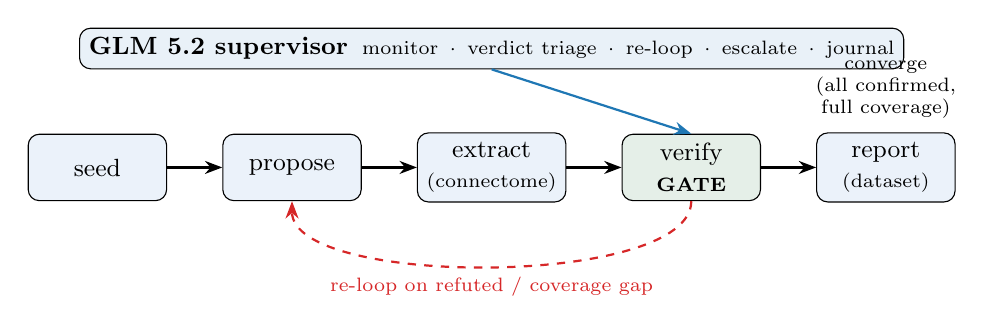
\begin{tikzpicture}[
  font=\small,
  stage/.style={draw,rounded corners,fill=stagebox,minimum height=2.4em,minimum width=5.0em,align=center},
  gate/.style={draw,rounded corners,fill=confirm!12,minimum height=2.4em,minimum width=5.0em,align=center},
  arr/.style={-{Stealth[length=2.2mm]},thick},
]
\node[stage] (seed) {seed};
\node[stage,right=0.7cm of seed] (prop) {propose};
\node[stage,right=0.7cm of prop] (ext) {extract\\\scriptsize(connectome)};
\node[gate,right=0.7cm of ext] (ver) {verify\\\scriptsize\textbf{GATE}};
\node[stage,right=0.7cm of ver] (rep) {report\\\scriptsize(dataset)};
\draw[arr] (seed)--(prop); \draw[arr] (prop)--(ext); \draw[arr] (ext)--(ver); \draw[arr] (ver)--(rep);
% re-loop arc
\draw[arr,contra,dashed] (ver.south) .. controls +(0,-1.1) and +(0,-1.1) .. (prop.south)
  node[midway,below,contra,font=\scriptsize]{re-loop on refuted / coverage gap};
% supervisor
\node[draw,rounded corners,fill=ipsi!10,above=0.8cm of ext,minimum width=15.5em,align=center] (sup)
  {\textbf{GLM 5.2 supervisor}\;\;\scriptsize monitor $\,\cdot\,$ verdict triage $\,\cdot\,$ re-loop $\,\cdot\,$ escalate $\,\cdot\,$ journal};
\draw[arr,ipsi] (sup.south) -- (ver.north);
\node[font=\scriptsize,above=0.05cm of rep,align=center] {converge\\(all confirmed,\\full coverage)};
\end{tikzpicture}%
}
\caption{\textbf{The closed-loop agentic tracing system.} A deterministic five-stage pipeline
(\ttt{seed}$\rightarrow$\ttt{propose}$\rightarrow$\ttt{extract}$\rightarrow$\ttt{verify}$\rightarrow$\ttt{report})
is supervised by a language-model agent. The \ttt{verify} stage is a hard gate: a round certifies only
if no claim is refuted and bilateral coverage is complete; otherwise the loop re-proposes and re-runs.
The supervisor reasons over verdicts but cannot alter them.}
\label{fig:system}
\end{figure}

\section{Verifying and resolving the wing-steering output}

We instantiated the system on the source paper's two named functional endpoints (DNbe001, DNp26),
expanded to the seven figure-driven wing-steering DN types, and traced
DN $\rightarrow$ motor neuron $\rightarrow$ wing muscle across both wings in the male whole-CNS
connectome (MCNS v1.0), with the brain-side figure$\rightarrow$DN edges drawn from FlyWire FAFB
(materialization 783). Wing laterality is defined relative to each DN's own soma side: a motor neuron
is on the \emph{ipsilateral} wing if it shares the DN's side, otherwise \emph{contralateral}; the
bilateral power muscles (DLM/DVM) are excluded from the steering denominator, following the source paper.

\subsection{Independent reproduction of the source paper's S14/S15}

The system re-derived the source paper's wing-laterality table (its S14) for all seven DNs directly
from the connectome. Every reported value is reproduced (Table~\ref{tab:s14}): each DN's ipsilateral
fraction matches to within rounding, the categorical wing assignment matches exactly, and the per-DN
steering-synapse totals are identical (e.g.\ DNa04 $908$, DNbe001 $1181$, DNge107 $1044$, DNbe005
$459$). DNp26's steering-muscle targets likewise reproduce the source paper's S15 exactly
(Table~\ref{tab:s15}: contralateral \ttt{hg1}~$=122$, \ttt{i1}~$=105$, \ttt{hg2}~$=117$, \ttt{b3}~$=28$).
This is an independent confirmation of the source paper's motor-side claims, and the verified baseline
on which the per-edge dataset below rests.

\begin{table}[t]
\centering
\small
\caption{\textbf{Per-DN wing laterality across both wings (independent reproduction of S14).} Computed
from MCNS by the agentic system; all seven rows reproduce the source paper's S14 values (ipsi.\ fraction
and wing assignment match; steering-synapse totals are identical). ``Wing'' is assigned ipsilateral if
ipsi.\ frac.\ $\geq 0.6$, contralateral if $\leq 0.4$, else bilateral.}
\label{tab:s14}
\begin{tabular}{l r r r r l}
\toprule
\textbf{DN} & \textbf{steering syn.} & \textbf{ipsi.\ syn.} & \textbf{contra.\ syn.} & \textbf{ipsi.\ frac.} & \textbf{wing} \\
\midrule
DNbe001 & 1181 & 619 & 562 & 0.524 & bilateral \\
DNge107 & 1044 & 609 & 435 & 0.583 & bilateral \\
DNa04   &  908 & 903 &   5 & 0.994 & \textcolor{ipsi}{ipsilateral} \\
DNbe005 &  459 & 195 & 264 & 0.425 & bilateral \\
DNp26   &  386 &  87 & 299 & 0.225 & \textcolor{contra}{contralateral} \\
DNg32   &  313 &  10 & 303 & 0.032 & \textcolor{contra}{contralateral} \\
DNge094 &   37 &   0 &  37 & 0.000 & \textcolor{contra}{contralateral} \\
\bottomrule
\end{tabular}
\end{table}

\begin{table}[t]
\centering
\small
\caption{\textbf{DNp26 wing-steering muscle targets} (summed over both DNp26 cells), reproducing the
source paper's S15. The strongest targets are the contralateral first-basalar/axillary steering muscles
that set wing-stroke amplitude and angle.}
\label{tab:s15}
\begin{tabular}{l r l}
\toprule
\textbf{steering muscle} & \textbf{synapses} & \textbf{wing (rel.\ to DN)} \\
\midrule
\ttt{hg1} & 122 & contralateral \\
\ttt{hg2} & 117 & mixed (ipsi+contra) \\
\ttt{i1}  & 105 & contralateral \\
\ttt{b3}  &  28 & contralateral \\
\ttt{hg3} &   5 & contralateral \\
\bottomrule
\end{tabular}
\end{table}

\subsection{The per-edge bilateral dataset}

With the baseline verified, the system emitted the per-edge dataset underlying the source paper's
summary tables: \textbf{488} DN$\rightarrow$motor-neuron edges onto \textbf{139} motor neurons reaching
\textbf{69} muscles, with \textbf{both-wing coverage $=1.0$} and \textbf{chain completeness $=1.0$}---every
seed DN reaches wing-steering motor neurons on both wings through a closed
DN$\rightarrow$MN$\rightarrow$muscle chain, with no missing entries. Where S14 gives one
ipsilateral-fraction per DN, this dataset gives the individual edges that fraction is computed from
(pre/post identity, synapse count, and wing side per edge), and likewise resolves the per-muscle,
per-wing breakdown behind S15. The circuit it represents---from the source paper's retinotopic readout
through to wing musculature on both sides---is shown in Fig.~\ref{fig:circuit}.

The resolved map makes the behavioral logic concrete. The same retinotopic figure representation
issues a \emph{mixture} of motor commands (Table~\ref{tab:s14}): \textbf{bilateral} commands through
DNbe001 (ipsi.\ frac.\ $0.52$) and DNge107 ($0.58$); a \textbf{purely ipsilateral} command through
DNa04 ($0.99$); and \textbf{contralateral}, single-wing commands through DNp26 ($0.23$), DNg32
($0.03$), and DNge094 ($0.00$). A figure signal that is itself retinotopic (position-coded on the
LLPC1 sheet) is thus converted into a set of left-versus-right wing adjustments---the anatomical
substrate for a steering turn toward or away from a detected object. DNp26, the convergent steering
command at the end of the LLPC1$\rightarrow$Nod1 pathway, makes its strongest connections onto the
contralateral \ttt{hg1}/\ttt{i1}/\ttt{hg2} muscles, which modulate wing-stroke amplitude and angle:
an unbroken route from a motion-defined figure to a wing-specific behavioral output.

\begin{figure}[t]
\centering
\resizebox{\textwidth}{!}{%
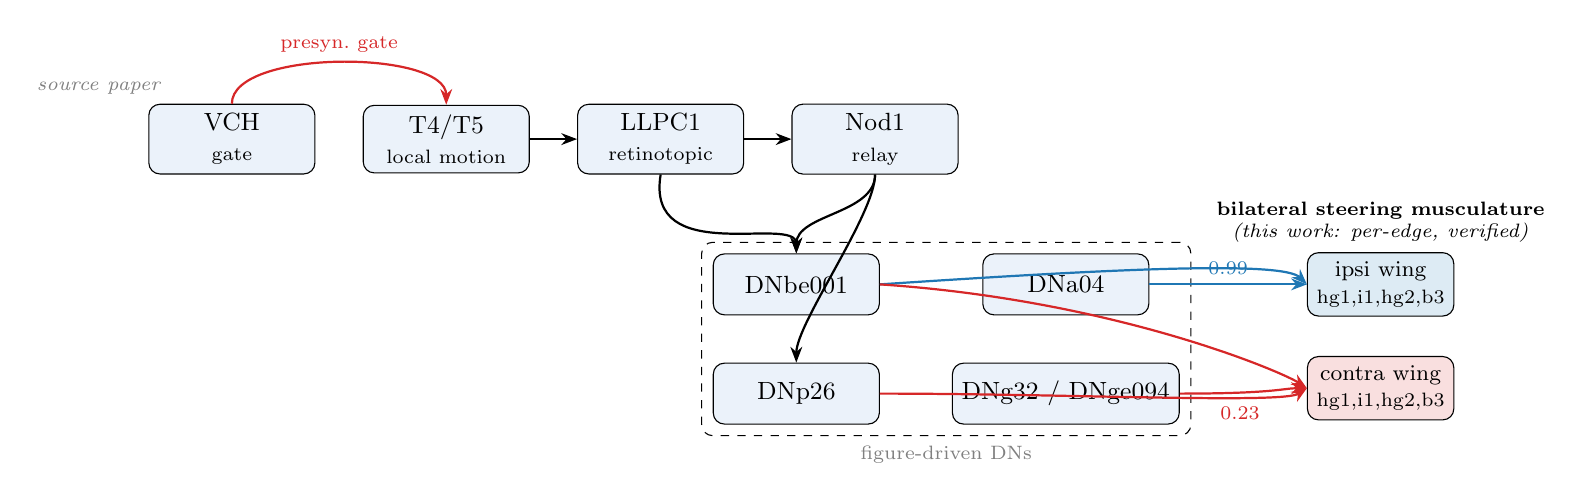
\begin{tikzpicture}[
  font=\small,
  node distance=6mm,
  cell/.style={draw,rounded corners,fill=stagebox,minimum height=2.2em,minimum width=6.0em,align=center},
  musc/.style={draw,rounded corners,minimum height=1.9em,minimum width=4.2em,align=center,font=\footnotesize},
  arr/.style={-{Stealth[length=2.0mm]},thick},
]
% brain side (from source paper)
\node[cell] (vch) {VCH\\\scriptsize gate};
\node[cell,right=of vch] (t45) {T4/T5\\\scriptsize local motion};
\node[cell,right=of t45] (llpc) {LLPC1\\\scriptsize retinotopic};
\node[cell,right=of llpc] (nod) {Nod1\\\scriptsize relay};
\draw[arr] (t45)--(llpc); \draw[arr] (llpc)--(nod);
\draw[arr,contra] (vch.north) .. controls +(0,0.7) and +(0,0.7) .. (t45.north)
  node[midway,above,font=\scriptsize,contra]{presyn.\ gate};
\node[font=\scriptsize,above left=0.0cm and -0.3cm of vch,gray] {\emph{source paper}};

% DN layer
\node[cell,below=1.0cm of nod,xshift=-1.0cm] (dnbe) {DNbe001};
\node[cell,below=of dnbe] (dnp) {DNp26};
\node[cell,right=1.3cm of dnbe] (dna) {DNa04};
\node[cell,below=of dna] (dng) {DNg32 / DNge094};
\draw[arr] (nod.south) .. controls +(0,-0.5) and +(0,0.5) .. (dnbe.north);
\draw[arr] (nod.south) .. controls +(0,-0.5) and +(0,0.5) .. (dnp.north);
\draw[arr] (llpc.south) .. controls +(-0.2,-1.2) and +(0,0.5) .. (dnbe.north);

% muscles bilateral
\node[musc,fill=ipsi!15,right=2.0cm of dna] (ipsiM) {ipsi wing\\\scriptsize hg1,i1,hg2,b3};
\node[musc,fill=contra!15,below=0.5cm of ipsiM] (contraM) {contra wing\\\scriptsize hg1,i1,hg2,b3};

\draw[arr,ipsi] (dna.east) -- (ipsiM.west) node[midway,above,font=\scriptsize,ipsi]{0.99};
\draw[arr,contra] (dnp.east) .. controls +(2.4,0) and +(-0.3,-0.2) .. (contraM.west)
  node[pos=0.7,below,font=\scriptsize,contra]{0.23};
\draw[arr,contra] (dng.east) .. controls +(1.2,0) and +(-0.3,0) .. (contraM.west);
\draw[arr,ipsi] (dnbe.east) .. controls +(3.0,0.2) and +(-0.3,0.3) .. (ipsiM.west);
\draw[arr,contra] (dnbe.east) .. controls +(3.0,-0.2) and +(-0.3,0.2) .. (contraM.west);
\node[font=\scriptsize,above=0.0cm of ipsiM,align=center] {\textbf{bilateral steering musculature}\\\scriptsize\emph{(this work: per-edge, verified)}};

\begin{scope}[on background layer]
\node[fit=(dnbe)(dnp)(dna)(dng),draw,dashed,rounded corners,inner sep=4pt,label={[font=\scriptsize,gray]below:figure-driven DNs}] {};
\end{scope}
\end{tikzpicture}%
}
\caption{\textbf{The figure--ground circuit through to bilateral wing musculature.} The brain-side
stages (VCH gate $\rightarrow$ T4/T5 $\rightarrow$ LLPC1 $\rightarrow$ Nod1) are from the source paper.
This work verifies and resolves the motor side at per-edge resolution: the seven figure-driven DNs are
traced through motor neurons to wing-steering muscles on \emph{both} wings (488 edges; the per-edge
wiring behind the source paper's S14/S15 summaries). Edge colors denote ipsilateral (blue) versus
contralateral (red) wing; numbers are ipsilateral synapse fractions. The same retinotopic figure signal
drives bilateral (DNbe001), ipsilateral (DNa04), and contralateral (DNp26, DNg32, DNge094) steering
commands.}
\label{fig:circuit}
\end{figure}

\subsection{Verification outcome}

The certified dataset carries \textbf{\textcolor{confirm}{26 confirmed}} claims,
\textbf{\textcolor{caveat}{3 confirmed-with-caveat}}, and \textbf{0 refuted} (Table~\ref{tab:verdicts}).
The three caveats are all from the soma-side permutation null on the most strongly lateralized DNs
(DNa04, DNp26, DNg32): the per-DN sample of steering motor neurons is small enough that the observed
wing bias---though anatomically unambiguous (e.g.\ DNa04 at $99.4\%$ ipsilateral)---is not formally
separable from a permutation null at the per-DN level. We report this honestly as a caveat rather than
suppressing it; it does not affect the laterality assignments, which match the source paper exactly.
No claim was refuted and coverage was complete, so the loop converged in a single round without
re-proposing.

\begin{table}[t]
\centering
\small
\caption{\textbf{Verification verdict summary} for the certified dataset. Two-track re-derivation plus
oracle cross-check against the source paper's S14/S15; laterality additionally tested against a
soma-side permutation null.}
\label{tab:verdicts}
\begin{tabular}{l r p{8.2cm}}
\toprule
\textbf{verdict} & \textbf{n} & \textbf{meaning} \\
\midrule
\textcolor{confirm}{\textbf{Confirmed}} & 26 & value matches the source paper / re-derives consistently on both tracks \\
\textcolor{caveat}{\textbf{Confirmed w/ caveat}} & 3 & per-DN laterality bias not separable from the permutation null at small sample (DNa04, DNp26, DNg32) \\
\textbf{Refuted} & 0 & --- \\
\bottomrule
\end{tabular}
\end{table}

\section{Discussion}

The source paper traced a figure--ground circuit from a retinotopic sensory representation to wing-steering
descending neurons and reported, in its supplementary tables, each figure-driven DN's wing-steering output
split by wing. This work independently confirms that motor-side result and renders it at per-edge
resolution. Two contributions stand together; we are careful not to overstate either.

\textbf{Scientifically}, we provide an independent reproduction plus a per-edge map. The source paper's
S14 (per-DN ipsi/contra fractions) and S15 (DNp26 muscle targets) are reproduced exactly from the
connectome---an external check on the motor-side claims---and we additionally emit the underlying
per-edge dataset (488 DN$\rightarrow$MN edges, 139 motor neurons, 69 muscles, both-wing coverage) that
those summary tables aggregate. We do \emph{not} claim to have discovered bilateral structure absent
from the source paper: S14 already reports the wing split for these DNs. What is new here is the
verification and the edge-level resolution---the specific motor neurons and muscles, per wing, behind
each published fraction. With that map in hand, the behavioral logic is concrete: the figure-driven DN
population converts a single retinotopic figure signal into a structured set of bilateral (DNbe001),
ipsilateral (DNa04), and contralateral single-wing (DNp26, DNg32, DNge094) steering commands onto
identified wing muscles---the anatomical form required to turn toward or away from a detected object.

\textbf{Methodologically}, the result was produced by a closed-loop agentic system whose defining
feature is that it cannot certify a result it has not verified: the gate fails any round with a refuted
claim or incomplete coverage, the supervising model is structurally barred from altering verdicts, and
the per-edge dataset is emitted only after the source paper's summary values are reproduced. The
deterministic pipeline guarantees progression; the language-model layer supervises, triages, and reports.
This pairing---verifiable connectome tracing under autonomous, steerable supervision---offers a template
for independently checking and edge-resolving other connectomic circuit claims at scale, with an
anchor-then-resolve discipline that keeps the output faithful to its source.

\paragraph{Data and reproducibility.} All claims derive from public connectomic resources: FlyWire FAFB
(materialization 783) for the brain side and the male whole-CNS connectome (MCNS v1.0) for the motor
side. The certified dataset (\ttt{muscular\_projection\_dataset.json}), the per-claim verdict ledger
(\ttt{verification\_results.json}), the bilateral split, motor-target, and muscle-assignment tables, and
the agentic tracing system itself are committed under \mbox{\ttt{5 - Muscular Projection/}} in the
project repository.

\end{document}
